
\chapter{Ultrasonic test results}

\section{Range test (No motion)} 

\begin{figure} [h!]
  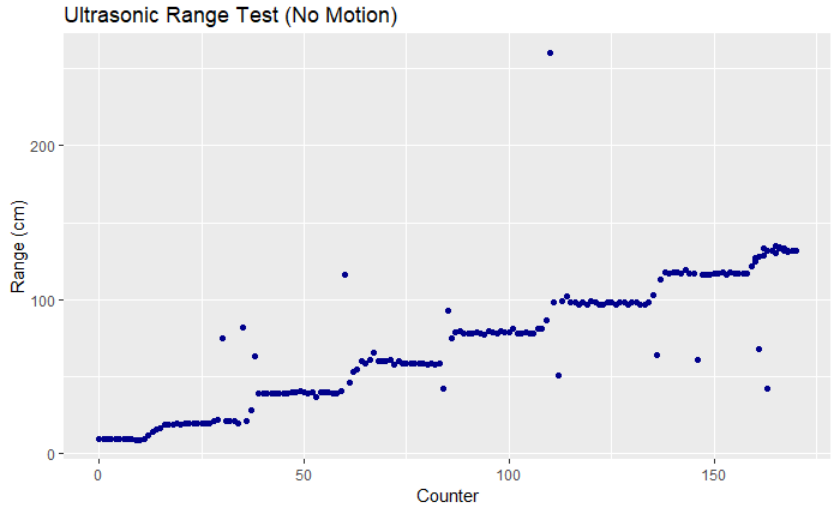
\includegraphics[width=\linewidth]{fig/test1}
  \caption{Ultrasonic range test (no motion)}
  \label{fig:test1}
\end{figure}

We did a ultrasonic range test where we placed a object in front of the ultrasonic sensor and moved it back \ref{fig:test1}. The test result shows that we got some outliers, but overall the ultrasonic sensor was fairly accurate.

\newpage

\section{Ultrasonic range test (motion)} 

\begin{figure} [h!]
  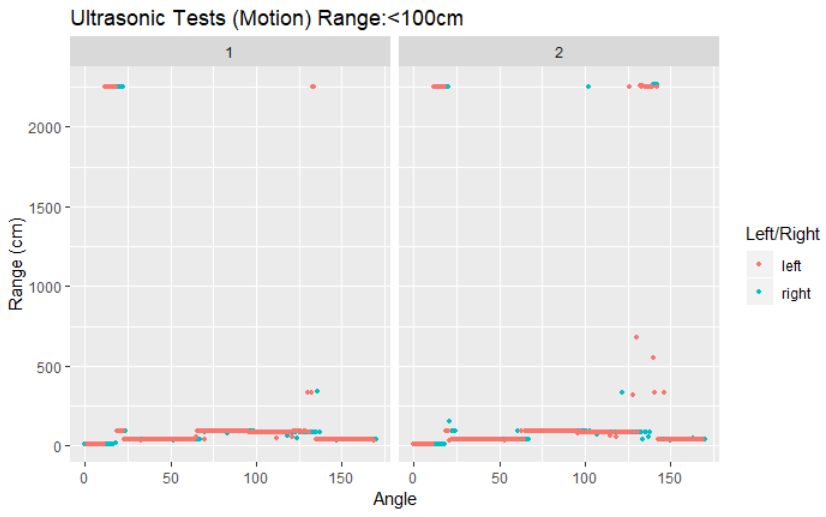
\includegraphics[width=\linewidth]{fig/test2}
  \caption{Ultrasonic range test (motion)}
  \label{fig:test2}
\end{figure}

This test shows how accurate the sensor is when moving from $0$ to $170$ (right) then $170$ to $0$ (left) two times, $Test 1$ and $Test 2$. As seen on \ref{fig:test2}.

The test\ref{fig:test2} should show us again that the sensor is accurate enough for us to work with, even though we got some strange outliers, like in $Test 2$ between Angle $130$ and $150$. The outliers that are $2500 cm$ is when the sensor didn't hit an object. 

\newpage

\section{Ultrasonic range test (motion) Range:<100 cm} 

\begin{figure} [h!]
  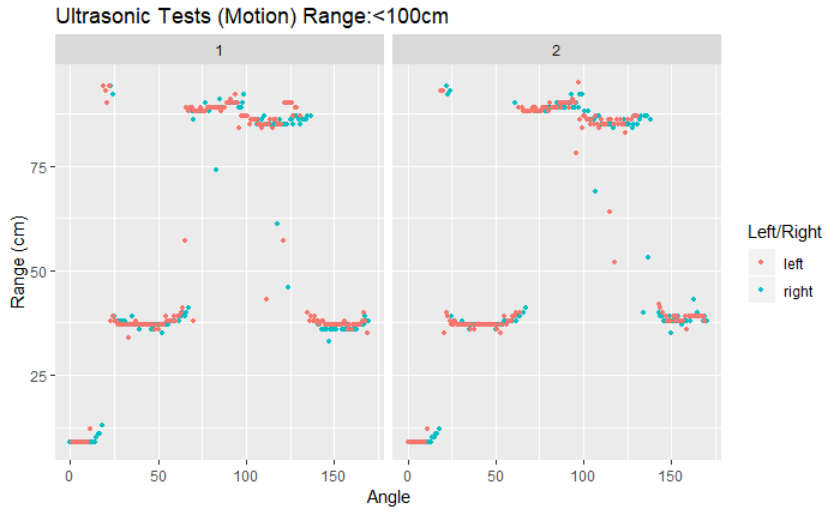
\includegraphics[width=\linewidth]{fig/test3}
  \caption{Ultrasonic range test (motion) Range:<100 cm}
  \label{fig:test3}
\end{figure}

In \ref{fig:test3} we only show everything that is below $100 cm$. This is to show a better image of the results.

\newpage

\section{Ultrasonic range tests separated (motion) Range:<100 cm} 

\begin{figure}[!h]
    \centering
    \subfloat[Test 1]{{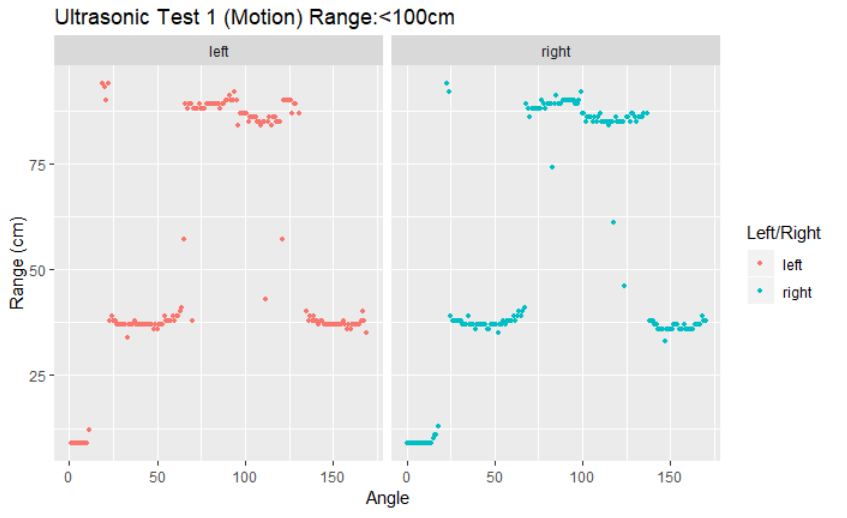
\includegraphics[width=5cm]{fig/test4} }}%
    \qquad
    \subfloat[Test 2]{{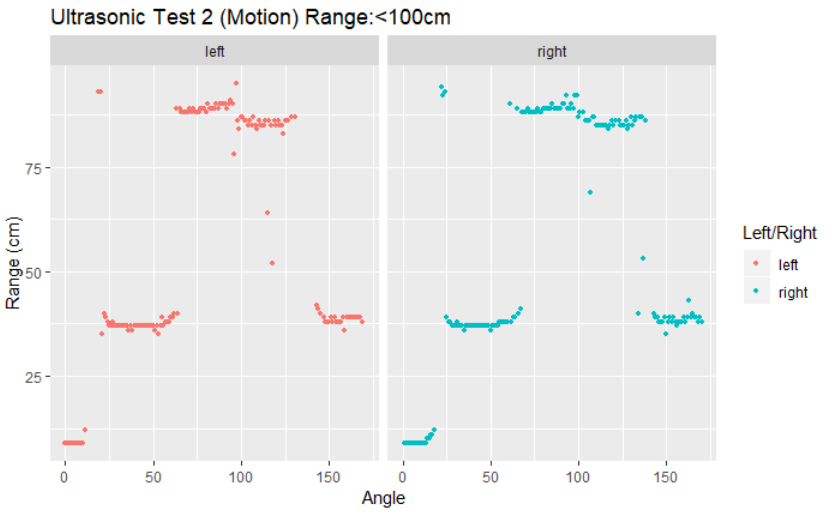
\includegraphics[width=5cm]{fig/test5} }}%
    \caption{Ultrasonic range tests separated (motion) Range:<100 cm}%
    \label{fig:test45}%
\end{figure} 

Here everything is separated. If the ultrasonic sensor was $100\%$ accurate, all the four images should look the same. As we can see to look quite similar, at least similar enough for us to be happy with the test results. 

We can also point out that a reason for the test results not looking exactly the same where the temperature readings. Sometimes we also got strange temperature readings and since we took a reading every $10$ degree, this could have a small effect on the results.
